\documentclass[a4paper]{article}
\usepackage[margin=1in]{geometry}%设置边距,符合Word设定
\usepackage{amssymb,amsfonts,amsmath,amsthm}
\usepackage{ctex}
\usepackage{setspace}
\usepackage{lipsum}
\usepackage{graphicx}%插入图片
\graphicspath{{Figures/}}%文章所用图片在当前目录下的 Figures目录

\usepackage{hyperref} % 对目录生成链接,注:该宏包可能与其他宏包冲突,故放在所有引用的宏包之后
\hypersetup{colorlinks = true,  % 将链接文字带颜色
	bookmarksopen = true, % 展开书签
	bookmarksnumbered = true, % 书签带章节编号
	pdftitle = 第三章扩展作业, % 标题
	pdfauthor = 刘正浩 2019270103005} % 作者

%\renewcommand{\contentsname}{\centerline{Contents}} %经过设置word格式后,将目录标题居中


\title{\heiti\zihao{2} 第三章扩展作业}
\author{\songti 刘正浩 2019270103005}
\date{2021年5月31日}


\begin{document}
	\maketitle
	\thispagestyle{empty}

	%\begin{abstract}
	%	\lipsum[2]
	%\end{abstract}

	\tableofcontents

	\section{第一题}
		\begin{figure}[htbp]
			\centering
			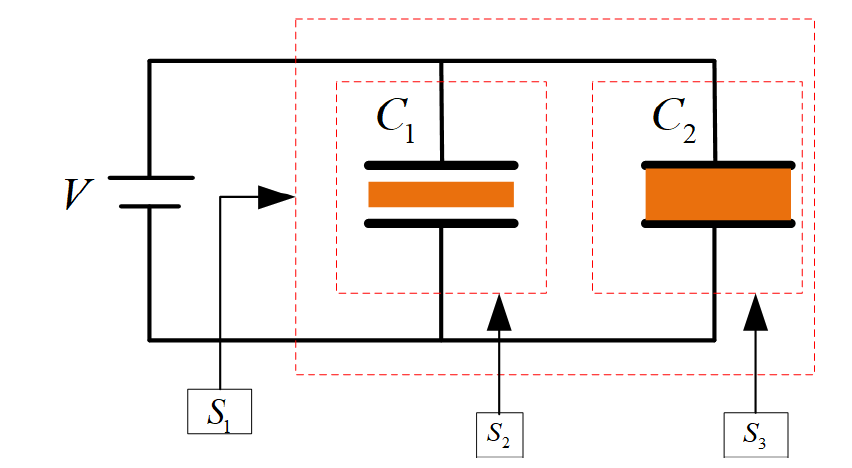
\includegraphics[scale=0.5]{1.png}
			\caption{电容与电压源组成的电路}
		\end{figure}
		已知电介质非理想(同时具有有限大小的电导率和介电常数)。设电介质的介电常数为$\varepsilon$,电导率为$\sigma$。电容器两极板间厚度为$d$,极板面积为$S$。\par
		首先分析$S_2$区域。设$S_2$区域中电介质的厚度为$d_1$,极板上的电荷量为$Q$。易知电容器中的问题为一维问题。应用高斯定理积分方程可知
		\begin{equation}
			\vec{D}(\vec{r}) = \vec{e_z} D(z) = \vec{e_z} \frac{Q}{S}
		\end{equation}
		故可得两极板间电压表达式
		\begin{equation}
			V = E_1(z)d_1 + E(z)(d - d_1) = \frac{Q}{S} \bigg( \frac{d_1}{\varepsilon} + \frac{d - d_1}{\varepsilon_0} \bigg)
		\end{equation}\par
		根据电容的表达式可知,
		\begin{equation}
			C_{S_2} = \frac{Q}{V} = \frac{\varepsilon_0 \varepsilon S}{\varepsilon_0 d_1 + \varepsilon (d-d_1)}
		\end{equation}\par
		由于真空电导率为0,故电阻为无穷大。\par
		在电介质区域中,
		\begin{equation}
			E_{1S_2} = \frac{Q}{\varepsilon S} = \frac{\varepsilon_0 V}{\varepsilon_0 d_1 + \varepsilon (d-d_1)}
		\end{equation}
		在真空区域中,
		\begin{equation}
			E_{2S_2} = \frac{Q}{\varepsilon_0 S} = \frac{\varepsilon V}{\varepsilon_0 d_1 + \varepsilon (d-d_1)}
		\end{equation}\par
		电容所包含的能量可以直接用电容包含能量的公式进行计算。
		\begin{equation}
			W_{S_2} = \frac{1}{2} C V^2 = \frac{\varepsilon_0 \varepsilon S V^2}{2[\varepsilon_0 d_1 + \varepsilon (d-d_1)]}
		\end{equation}
		功率
		\begin{equation}
			P_{S_2} = \frac{\mathrm{d} W_C}{\mathrm{d} t} = 0
		\end{equation}
		这很好理解,因为电容器中并没有电流通过,也就没有电功率。\par
		接着来分析$S_3$区域。仍设极板上的电荷量为$Q$。此电容器中的问题仍为一维问题。应用高斯定理积分方程。、
		\begin{equation}
			\vec{D}(\vec{r}) = \vec{e_z} D(z) = \vec{e_z} \frac{Q}{S}
		\end{equation}\par
		带入电压表达式。
		\begin{equation}
			V = E_1(z) d = \frac{Q}{S} \frac{d}{\varepsilon}
		\end{equation}\par
		根据电容的表达式可知
		\begin{equation}
			C_{S_3} = \frac{Q}{V} = \frac{\varepsilon S}{d}
		\end{equation}\par
		由静电比拟法,可知此电容器的电阻值。
		\begin{equation}
			R_{S_3} = \frac{1}{\frac{\sigma S}{d}} = \frac{d}{\sigma S}
		\end{equation}\par
		电场强度为
		\begin{equation}
			E_{S_3} = \frac{Q}{\varepsilon S} = \frac{\varepsilon V}{d}
		\end{equation}\par
		在此区域中,能量由电容存储
		\begin{equation}
			W_{S_3} = W_C = \frac{1}{2} C V^2 = \frac{\varepsilon S V^2}{2d}
		\end{equation}
		总功率为电流热效应的功率
		\begin{equation}
			P_{S_3} = UI = \frac{V^2}{R} = \frac{\sigma S V^2}{d}
		\end{equation}\par
		最后分析$S_1$区域。\par
		电场情况已由上面内容中给出。\par
		根据电路的相关知识,
		\begin{equation}
			C = C_{S_2} + C_{S_3} = \frac{\varepsilon_0 \varepsilon S}{\varepsilon_0 d_1 + \varepsilon (d-d_1)} + \frac{\varepsilon S}{d}
		\end{equation}
		\begin{equation}
			R = R_{S_2} || R_{S_3} = R_{S_3} = \frac{d}{\sigma S}
		\end{equation}\par
		能量
		\begin{equation}
			W = W_{S_2} + W_{S_3} = \frac{\varepsilon_0 \varepsilon S V^2}{2[\varepsilon_0 d_1 + \varepsilon (d-d_1)]} + \frac{\varepsilon S V^2}{2d}
		\end{equation}
		功率
		\begin{equation}
			P = P_{S_2} + P_{S_3} = 0 + \frac{\sigma S V^2}{d} = \frac{\sigma S V^2}{d}
		\end{equation}

\end{document}